\documentclass[a4paper,oneside,12pt]{book}
%% === nezbytné balíčky:
\usepackage[T1]{fontenc}    % kódování písma
%\usepackage[IL2]{fontenc}  % kódování písma
\usepackage{graphicx}
\usepackage[utf8]{inputenc}     % vstupní znaková sada tohoto dokumentu: UTF-8
%\usepackage[cp1250]{inputenc}  % vstupní znaková sada tohoto dokumentu: Windows 1250
%\usepackage[latin2]{inputenc}  % vstupní znaková sada tohoto dokumentu: ISO Latin 2
\usepackage{siunitx}
\usepackage[czech]{babel} % česky psaná práce, typografická pravidla. Překládejte pomocí "latex.exe" nebo "pdflatex.exe"
%\usepackage{czech} % česky psaná práce. Překládejte pomocí "pdfCSlatex.exe" ("cslatex.exe" asi bude mít problém s balíkem geometry)
\usepackage{hhline} % Add the hhline package
\usepackage[a4paper, hmarginratio=3:2]{geometry} % využití A4 stránky a nastavení okrajů (u vazby bude širší)
\usepackage{afterpage}
\usepackage{caption}
\usepackage{pdfpages} % pokud nemáte formulář "Zadání bak./dipl. práce" naskenovaný jako PDF, tak ZAKOMENTUJTE
\usepackage[hidelinks]{hyperref} % v PDF budou klikací odkazy ("hidelinks" je nebude rámovat)
%% === balíčky, které se mohou hodit:
%\usepackage{encxvlna} % postará se o spojky a předložky, které dle českých pravidel nesmí být na konci řádku. Dokumentace: http://texdoc.net/texmf-dist/doc/generic/encxvlna/encxvlna.pdf (chová se správně k "vnitřku" listings?)

\usepackage{graphicx} % balíček pro vkládání rastrových grafických souborů (PNG apod.)
%\usepackage{epsfig} % balíčky pro vkládání grafických souborů typu EPS
\usepackage{float} % rozšířené možnosti umístění obrázků

%\usepackage{caption} % pro popisky obrázků, tabulek atd.

\usepackage{tabularx} % rozšířené možnosti tabulek
%\usepackage{tabu} % jiný balík pro rozšířené možnosti tabulek

\usepackage{listings}  % balíček vhodný pro ukázky zdrojového kódu v~textu práce/příloh. Nutno nastavit! http://ftp.cvut.cz/tex-archive/macros/latex/contrib/listings/listings.pdf
\usepackage{amsmath} % balíček pro pokročilou matematickou sazbu
%\usepackage{color} % pro možnost barevného textu
%\usepackage{fancybox} % umožňuje pokročilé rámečkování

%\usepackage{index} % nutno použít v případě tvorby rejstříku balíčkem makeindex
%\newindex{default}{idx}{ind}{Rejstřík} % zavádí rejstřík v případě použití balíku index


\frenchspacing % za větou bude mezislovní mezera (v anglických textech je mezera za větou delší)
\widowpenalty=1000 % "síla" zákazu vdov (= jeden řádek ze začátku odstavce na konci stránky)
\clubpenalty=1000 % "síla" zákazu sirotků (= jeden řádek/slovo z konce odstavce samostatně na začátku stránky)
\brokenpenalty=1000 % "síla" zákazu zlomu stránky za řádkem, který má na konci rozdělené slovo

\topmargin=-15mm      % horní okraj trochu menší
\textwidth=150mm      % šířka textu na stránce
\textheight=240mm     % "výška" textu na stránce


\pagenumbering{arabic} % číslování stránek arabskými číslicemi
\pagestyle{plain}      % stránky číslované dole uprostřed

\parindent=0pt % odsazení 1. řádku odstavce
\parskip=7pt   % mezera mezi odstavci

\newcommand{\ti}{\textit} % zkrácený příkaz pro kurzívu
\newcommand{\tb}{\textbf} % zkrácený příkaz pro tučné písmo








%% --- zde jsou zavedeny některé "konstanty" - některé musíte změnit! --- %%
\newcommand{\cvut}{České vysoké učení technické v~Praze}
\newcommand{\fjfi}{Fakulta stavební}
\newcommand{\ksi}{Katedra geomatiky}
\newcommand{\program}{Geodézie a kartografie} % změňte, pokud máte jiný stud. program
\newcommand{\obor}{} % změňte, pokud máte jiný obor

\newcommand{\druh}{Diplomová práce} % nebo "Diplomová práce"
\newcommand{\woman}{} % pokud jste ŽENA, ZMĚŇTE na: ...{\woman}{a} (je to do Prohlášení)

\newcommand{\logoCVUT}{
\includegraphics{pictures/symbol_cvut_konturova_verze_cb.pdf}} % logo ČVUT -- podle grafického manuálu ČVUT platného od prosince 2016. Pokud nevyhovuje PDF-verze, tak použijte jinou variantu loga: https://www.cvut.cz/logo-a-graficky-manual -> "Symbol a logo ČVUT v Praze"). Pokud chcete logo úplně vynechat, zadejte místo "\includegraphics{...}" text "\vspace{35mm}"

% přesně podle formuláře "Zadání bak./dipl. práce" VYPLŇTE:
\newcommand{\nazevcz}{Vývoj zásuvného modulu QGIS pro určení využití území a potřeby analýz odtokových poměrů}    % český název práce (přesně podle zadání!)
\newcommand{\nazeven}{Development of a QGIS Plugin for Land Use Determination and Purposes of Runoff Analysis}          % anglický název práce (přesně podle zadání!)
\newcommand{\autor}{Bc. Josef Jehlička}   % vyplňte své jméno a příjmení (s akademickým titulem, máte-li jej)
\newcommand{\vedouci}{Ing. Martin Landa, Ph.D. } % vyplňte jméno a příjmení vedoucího práce, včetně titulů, např.: Doc. Ing. Ivo Malý, Ph.D.
\newcommand{\druhyvedouci}{doc. Ing. Petr Kavka, Ph.D.}
\newcommand{\pracovisteVed}{\ksi, \fjfi, \cvut} % ZMĚŇTE, pokud vedoucí Vaší práce není z KSI
\newcommand{\konzultant}{--} % POKUD MÁTE určeného konzultanta, NAPIŠTE jeho jméno a příjmení
\newcommand{\pracovisteKonz}{--} % POKUD MÁTE konzultanta, NAPIŠTE jeho pracoviště

% podle skutečnosti VYPLŇTE:
\newcommand{\rok}{2025}  % rok odevzdání práce (jen rok odevzdání, nikoli celý akademický rok!)
\newcommand{\kde}{Praze} % studenti z Děčína ZMĚNÍ na: "Děčíně" (doplní se k "prohlášení")

\newcommand{\klicova}{Klíčová slova}   % zde NAPIŠTE česky max. 5 klíčových slov
\newcommand{\keyword}{Key words}       % zde NAPIŠTE anglicky max. 5 klíčových slov (přeložte z češtiny)
\newcommand{\abstrCZ}{Popis práce česky}    % zde NAPIŠTE abstrakt v češtině (cca 7 vět, min. 80 slov)
\newcommand{\abstrEN}{Popis práce anglicky} % zde NAPIŠTE abstrakt v angličtině

\newcommand{\prohlaseni}{Prohlašuji, že jsem diplomovou práci s názvem "Vývoj QGIS zásuvného modulu pro potřeby výpočtu objemu přímého odtoku metodou SCS-CN“ vypracoval samostatně s odborným vedením pana Ing. Martina Landy, Ph.D a doc. Ing. Petra Kavky, Ph.D. Použitá literatura a další podklady, které byly použity pro tuto diplomovou práci, jsou uvedeny v seznamu literatury. 
} % text prohlášení můžete mírně upravit :-)

\newcommand{\podekovani}{Tímto bych chtěl poděkovat } % NAPIŠTE poděkování, např. svému vedoucímu:
% Děkuji Ing. Eleonoře Krtečkové, Ph.D. za vedení mé bakalářské práce a za podnětné návrhy, které ji obohatily.
% NEBO:
% Děkuji vedoucímu práce doc. Pafnutijovi Snědldítětikaši, Ph.D. za neocenitelné rady a pomoc při tvorbě bakalářské práce.













\begin{document}
%%%%%%%%%%%% TITULNÍ STRANA -- na následujících cca 30 řádků NESAHEJTE!!!  Generuje se AUTOMATICKY %%%%%%%%%%%%
\thispagestyle{empty}

\begin{center}
	{\LARGE
		\cvut\par
		\fjfi
	}
    \vspace{10mm}

    \begin{tabular}{c}
		\tb{\ksi} \\[3pt]   
		\tb{Program: \program}\\
    \end{tabular}

   \vspace{10mm} \logoCVUT \vspace{15mm} 

   {\huge \tb{\nazevcz}\par}
   \vspace{5mm}   
   {\huge \tb{\nazeven}\par}
   
   \vspace{15mm}
   {\Large \MakeUppercase{\druh}}

   \vfill
   {\large
    \begin{tabular}{ll}
    Vypracoval: & \autor\\
    Vedoucí práce: & \vedouci\\
    & \druhyvedouci \\
    Rok: & \rok
    \end{tabular}
   }
\end{center}



%%%%%%%%%%%% ZADÁNÍ PRÁCE %%%%%%%%%%%%
% Zadání (podepsané děkanem!) musíte NASKENOVAT. Ideálně jako 2stránkové PDF (soubor "zadani_cele.pdf"). 
% Před svázáním to v jednom výtisku VYMĚNÍTE ZA ORIGINÁLNÍ ZADÁNÍ (podepsané děkanem fakulty)!
\newpage  % SEM NESAHEJTE!
\thispagestyle{empty} % SEM NESAHEJTE!

%% zde podle toho, jak jste zadání naskenovali, VYBERTE variantu A, B nebo C:
%
% --- varianta A: zadání naskenované jako 2stránkové PDF:




 % 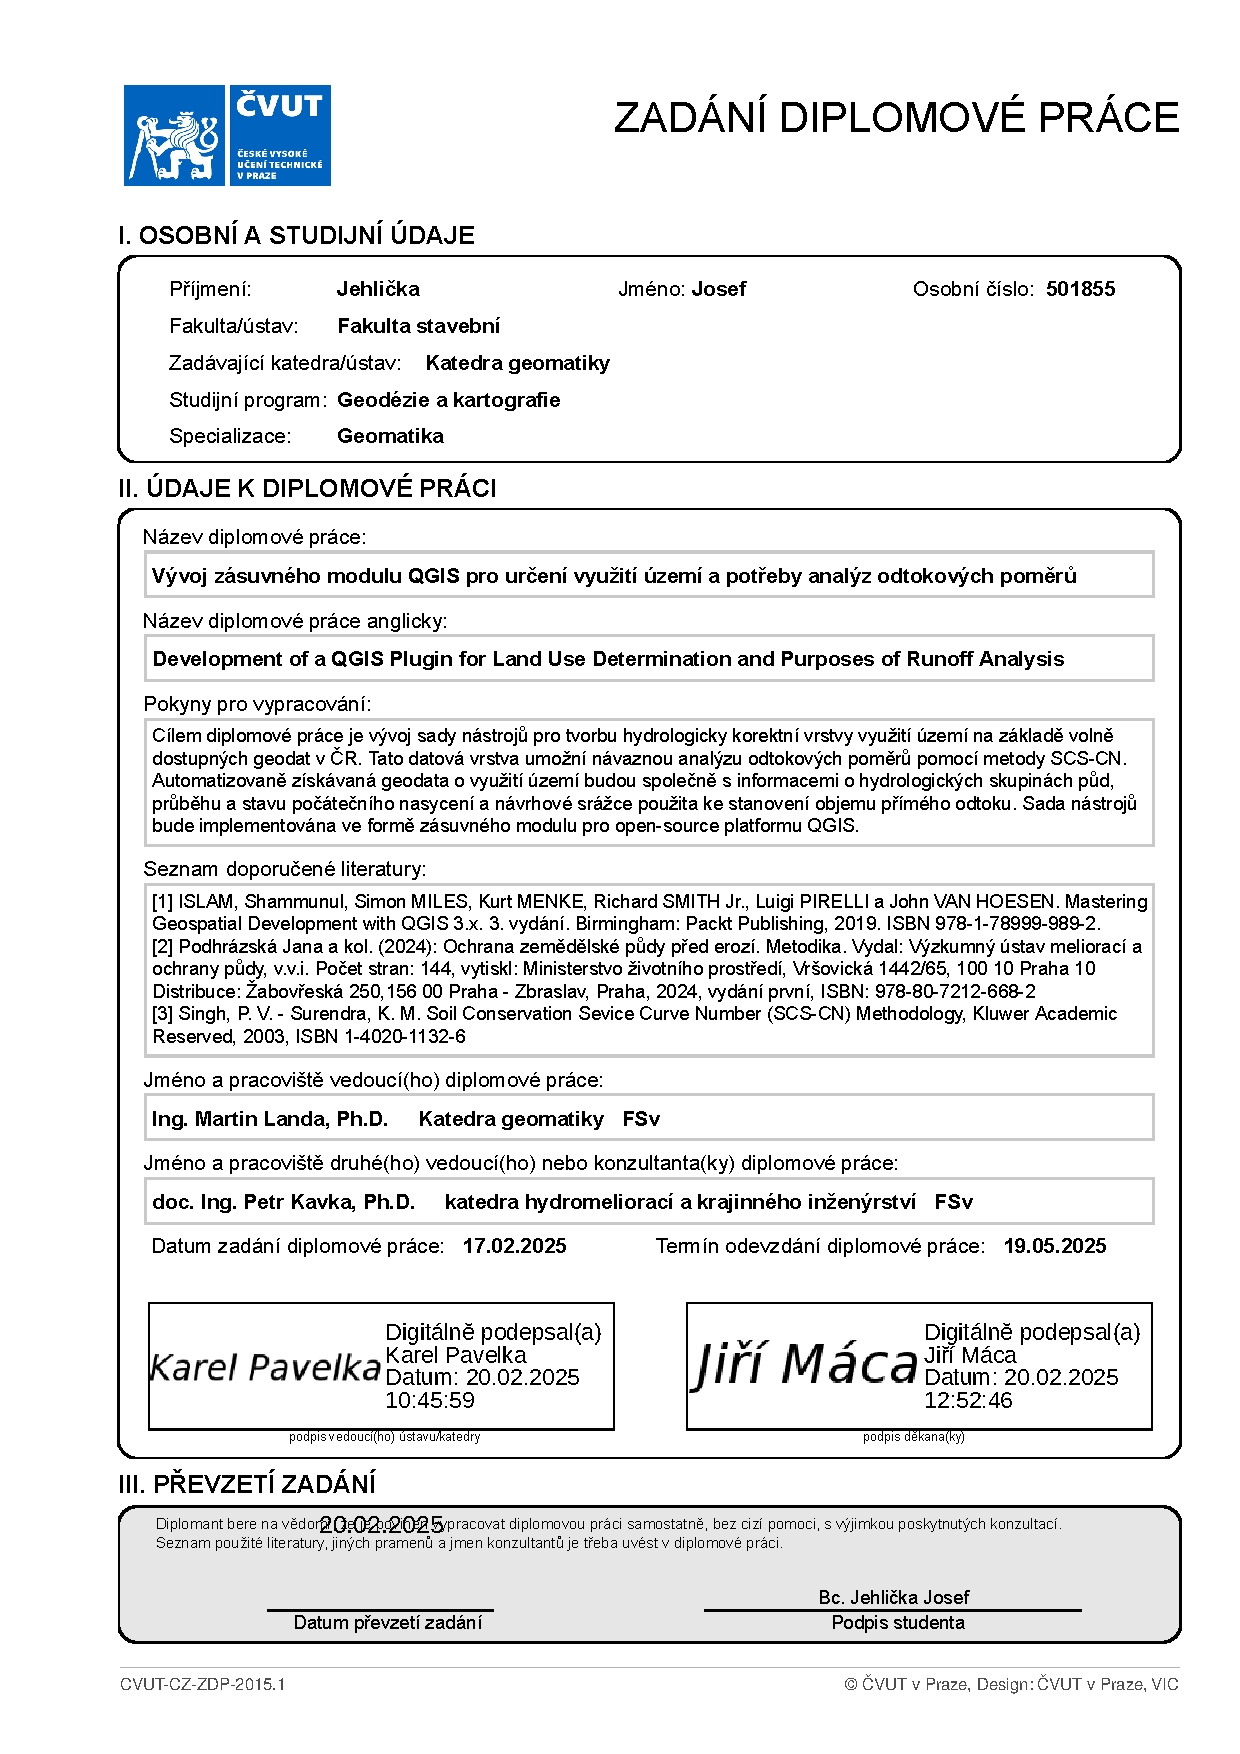
\includepdf[pages={1}]{zadani_cele.pdf} % NAHRAĎTE správným souborem! <<<<<<<<<<<<<<<<<<<<<<<<<





%
%% --- varianta B: zadání naskenované jako jednotlivé stránky:
%\includepdf[pages={1}]{zadani1.pdf} % 1. strana zadání v PDF
%\includepdf[pages={1}]{zadani2.pdf} % 2. strana zadání v PDF
%
%% --- varianta C: zadání naskenované jako 2 samostatné obrázky:
%% 1. strana zadání
%\begin{center}
%     \includegraphics[width=1\textwidth]{zadani1.jpg}
%\end{center}
%% 2. strana zadání
%\newpage  % SEM NESAHEJTE!
%\thispagestyle{empty} % SEM NESAHEJTE!
%\begin{center}
%     \includegraphics[width=1\textwidth]{zadani2.jpg}
%\end{center}







% příprava:    (na následujících 8 řádků NESAHEJTE!)
\newbox\odstavecbox
\newlength\vyskaodstavce
\newcommand\odstavec[2]{%
    \setbox\odstavecbox=\hbox{%
         \parbox[t]{#1}{#2\vrule width 0pt depth 4pt}}%
    \global\vyskaodstavce=\dp\odstavecbox
    \box\odstavecbox}
\newcommand{\delka}{120mm} % šířka textů ve 2. sloupci tabulky

% použití přípravy:    % dovnitř "tabular" vůbec NESAHEJTE!

\section*{ABSTRAKT}
\begin{flushleft}
Tato práce popisuje vývoj zásuvného modulu open-source softwaru QGIS, který provádí přípravu dat a následnou analýzu odtoků SCS-CN  na automatizovaně získávaných volně dostupných geo datech v ČR jako jsou ZABAGED, LPIS, RÚIAN a data poskytovaná projektem rain.fsv.cvut.cz. Data jsou ohodnocena podle způsobu využití území a v kombinaci s daty hydrologických skupin půd a hodnotou úhrnu návrhové srážky vstupují do následné analýzy.
\end{flushleft}


\section*{KLÍČOVÁ SLOVA}
\begin{flushleft}
QGIS, SCS-CN, využití území, zásuvný modul, Python, odtok, povodí, GIS, ZABAGED, LPIS
\end{flushleft}


\section*{ABSTRACT}
\begin{flushleft}
This master's thesis describes the development of a plugin for the open-source software QGIS, which performs data preparation and subsequent runoff analysis using the SCS-CN method on automatically acquired freely available geodata in the Czech Republic, such as ZABAGED, LPIS, RÚIAN, and data provided by the rain.fsv.cvut.cz project. The data are evaluated based on land use and, in combination with data on hydrologic soil groups and the total design rainfall amount, serve as inputs for the subsequent analysis.
\end{flushleft}


\section*{KEY WORDS}
\begin{flushleft}
QGIS, SCS-CN, land use, plugin, Python, runoff, watershed, GIS, ZABAGED, LPIS
\end{flushleft}

















%%%%%%%%%%%% Prohlášení -- SEM NESAHEJTE! Generuje se automaticky z výše nastavených maker \kde{} a \prohlaseni{}. %%%%%%%%%%%%
\newpage % SEM NESAHEJTE!
\thispagestyle{empty}  % SEM NESAHEJTE!

~ % SEM NESAHEJTE!
\vfill % prázdné místo. SEM NESAHEJTE!
\vspace{1em}
\tb{Prohlášení} % SEM NESAHEJTE!

\vspace{1em} % vertikální mezera. SEM NESAHEJTE!
\prohlaseni

\vspace{2em}  % SEM NESAHEJTE!
\hspace{-0.5em}\begin{tabularx}{\textwidth}{X c}  % SEM NESAHEJTE!
V \kde\ dne .................... &........................................ \\	% SEM NESAHEJTE!
	& \autor
\end{tabularx}	% SEM NESAHEJTE!







\newpage % SEM NESAHEJTE!
\thispagestyle{empty}  % SEM NESAHEJTE!

~
\vfill % prázdné místo


% -- následující kus kódu (do "%%%%%%%%%%%% ABSTRAKT") můžete odstranit, pokud nechcete psát poděkování:
\vspace{1em}
\tb{Poděkování}

\vspace{1em} % vertikální mezera
\podekovani
\begin{flushright}
\autor
\end{flushright}  % <------- tady končí stránka s poděkováním





\newpage
\chapter*{Obsah}




\newpage
\chapter*{Úvod} \label{uvod}

\newpage
\chapter{Meotda SCS-CN} \label{SCSCN}
\hspace{10mm} Metoda odtokových křivek (SCS-CN) se používá pro určení objemu přímého odtoku při návrhových přívalových deštích. Výhody této metody spočívají v její jednoduchosti a schopnosti reagovat na vlastnosti povodí jako je typ půdy či využití pozemku (land use). Metoda byla vyvinuta v roce 1954 a publikována v roce 1986 organizací USDA Natural Resources Conservation Service (dříve nazývána Soil Conservation Service). [1] Vývoj probíhal na empirických datech získaných v USA, nicméně později byla modifikována na různé typy využití pozemku typické i pro jiné podmínky. [2][3]

\hspace{10mm} Tato metoda může být využita i v menších částech jednotlivých povodí, jejichž rozloha by neměla překročit 10 $km^{2}$ a není vhodná pro výpočet odtoku z tání sněhu. V České republice se využívá hlavně pro návrhy protierozních opatření, a to v souladu s ČSN 75 1300. [4]

Výstupem metody CN křivek je hodnota efektivní srážkové výšky dle vzorce (1) [5]:


\begin{equation}
H_{0} = \frac{\displaystyle (H_{S} - I_{a})^{2}}{\displaystyle H_{S} - I_{a} + A}
\end{equation}

kde:
\begin{tabbing}
    \hspace{10mm} \= $H_{0}$ \hspace{5mm} \= je výška přímého odtoku (mm) \\
    \> $H_{s}$ \> je celkový srážkový úhrn (mm) \\
    \> $I_{a}$ \> je počáteční ztráta (mm) \\
    \> $A$ \> je maximální potenciální retence (mm)
\end{tabbing}

Hodnota počáteční ztráty ($I_{a}$) se určí jako:
\begin{equation}
I_{a} = \lambda A
\end{equation}

\hspace{10mm} Kde $\lambda$ je poměrový koeficient, který se v základu volí $0.2$. Tato hodnota byla empiricky odvozena na povodích na území USA. [3][5] Takto zvolená hodnota se stala jedním důvodem pro kritiku této metody. [1] \\

\hspace{10mm} Maximální potenciální retence ($A$) je dále určena na základě CN (curvature number) křivek ze vztahu [4] : 
\begin{equation}
A = 25,4 (\frac{1000}{CN}-10)
\end{equation}
\hspace{10mm} Hodnota CN se pohybuje mezi 0 (prakticky 30) až 100. Čím vyšší je hodnota CN, tím větší je pravděpodobnost, že dojde k povrchovému odtoku. Pokud se CN rovná nule, potom představuje teoretickou horní
hranici potenciální retence, což by znamenalo, že takové povodí je nekonečně propustné. [6]

\begin{figure}[ht] \label{obr1}
\centering
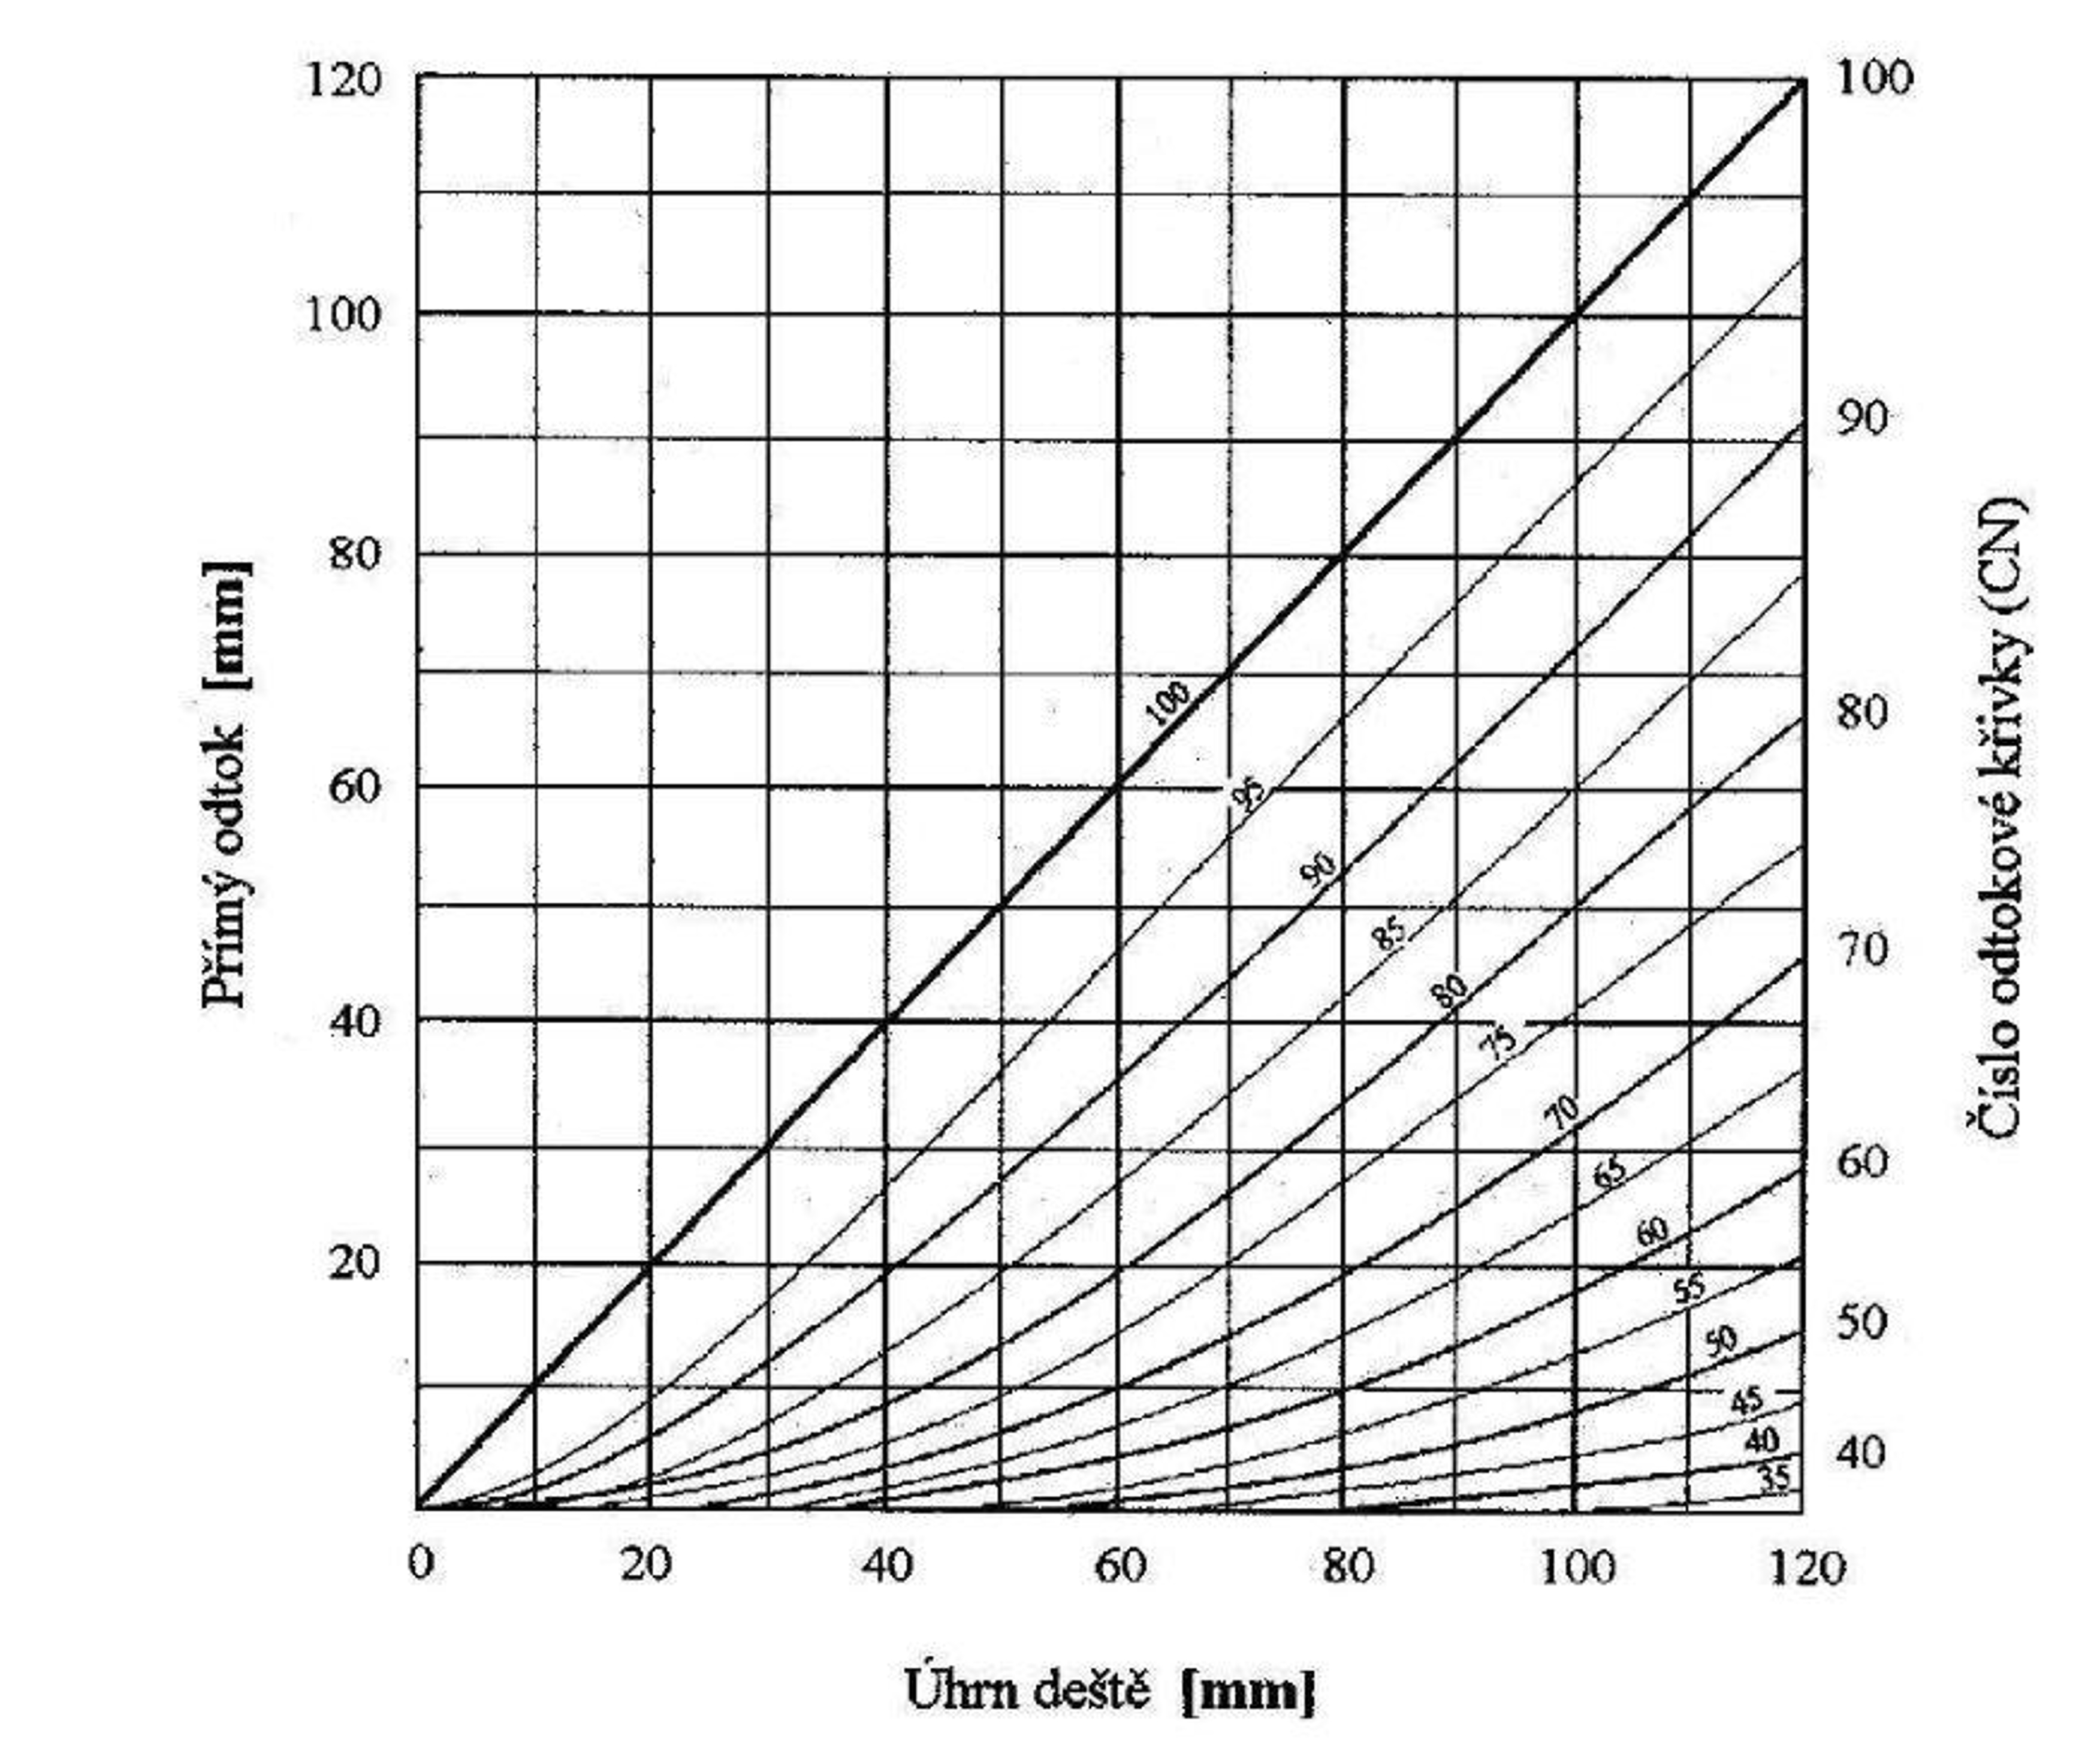
\includegraphics[height=12cm]{pictures/CNcurves.jpg}
\caption{ Závislost výšky přímého odtoku ($H_{o}$) na úhrnu deště($H_{S}$) a číslech odtokových křivek (CN) [4]}
\label{fig:example}
\end{figure}

 \hspace{10mm} Tato čísla jsou tabelována pro dvojici jevů. Těmi jsou hydrologické skupiny půd (HSP) a způsob využití území (land use) případně doplněn o počáteční vlhkostní podmínky. [6][7]

\hspace{10mm} Hydrologické skupiny půd (HSP) existují čtyři: A,B,C,D. Do těchto skupin se řadí půda dle minimálních rychlostí infiltrace vody do půdy bez pokryvu a po dlouhodobém nasycení.[4]
\begin{table}[htbp]
  \centering
  \caption{Tabulka rozdělení do hydrologických skupin půd (HSP) [4]} 
  \label{tab:HSP}
  \begin{tabular}{|c|p{6cm}|p{2.5cm}|p{2.5cm}|}
    \hline
    Skupina & Charakteristika hydrologických vlastností [m] & 
    Rychlost infiltrace [mm.min\textsuperscript{-1}] & Rychlost infiltrace [mm.den\textsuperscript{-1}] \\
    \hhline{=|=|=|=|}
    A & Půdy s vysokou rychlostí infiltrace i při úplném nasycení, zahrnující převážně hluboké, dobře až nadměrně odvodněné písky nebo štěrky. & > 0,12 & > 172 \\
    \hline
    B & Půdy se střední rychlostí infiltrace i při úplném nasycení, zahrnující převážně půdy středně hluboké až hluboké, středně až dobře odvodněné, hlinitopísčité až jílovitohlinité. & 0,06–0,12 & 86,4–172 \\
    \hline
    C & Půdy s nízkou rychlostí infiltrace i při úplném nasycení, zahrnující převážně půdy s málo propustnou vrstvou v půdním profilu a půdy jílovitohlinité až jílovité. & 0,02–0,06 & 28,8–86,4 \\
    \hline
    D & Půdy s velmi nízkou rychlostí infiltrace i při úplném nasycení, zahrnující především jíly s vysokou bobtnavostí, půdy s trvale vysokou hladinou podzemní vody, půdy s vrstvou jílu na povrchu nebo těsně pod ním a mělké půdy nad téměř nepropustným podložím. & < 0,02 & < 28,8 \\
    \hline
  \end{tabular}
  
\end{table}

% Různé zdroje půd (HSP) - velký rozdíl výsledků, je tam graf https://www.vodnihospodarstvi.cz/ArchivPDF/vh2022/vh_09-2022.pdf
\newpage
\chapter{QGIS} \label{qgis}
\hspace{10mm} QGIS (dříve známý jako Quantum GIS) je jeden z geografických informačních systémů (GIS), tj.  informační systém zabývající se informacemi, které se týkají jevů přidružených k místu vztaženému k Zemi.[8]

\begin{figure}[ht] \label{obr2}
\centering

\includegraphics[height=2cm]{pictures/qgis-logo.png}
\caption{Logo softwaru QGIS}
\label{fig:QGIS}
\end{figure}

\hspace{10mm} Tento software je podporován v prostředí Windows,Mac OS, Linux i Unix. Na rozdíl od komerčních alternativ, jako je například ArcGIS, je QGIS zcela zdarma k použití a řadí se mezi takzvaný otevřený software, který je spravován neziskovou organizací The Open Source Geospatial Foundation (OSGeo).

\begin{figure}[ht] \label{obr3}
\centering

\includegraphics[height=2cm]{pictures/Osgeo.png}
\caption{ Logo organizace OSGeo}
\label{fig:OSGEO}
\end{figure}

\hspace{10mm} OSGeo stojí i za řadou dalších projektů na poli otevřeného softwaru, jako jsou například:
\begin{itemize}
\item GRASS GIS 
\item gvSIG - GIS software
\item PROJ - knihovna pro tansformaci souřadnic a kartografických projekcí
\item GDAL/OGR - knihovna pro čtení a zápis GIS formátů
\item PostGIS - SQL pro práci s geoprostorovými daty
\item GeoServer - Serverová platforma umožňující publikaci prostorových dat 
\item OpenLayers - JavaScript knihovna pro tvorbu webových mapových aplikací
\end{itemize}


\hspace{10mm} QGIS funguje pod licencí GNU GPL a je postaven na knihovně Qt jazyka C++. QGIS vznikal iniciativou Garyho Shermana, který ji započal v roce 2002 jako prohlížecí software geoprostorových dat pro operační systém Linux. Jeho první verze vyšla až v roce 2009. [9]

 \section{Zásuvné moduly} \label{moduly}

\hspace{10mm} QGIS je pravidelně jeho vývojáři rozšiřován o nejrůznější funkce, často přejímané z dalších otevřených softwarů jako je například: GRASS GIS, GDAL nebo SAGA GIS.[10]

\hspace{10mm} Nespornou výhodou je i fakt, že jakákoliv nezávislá organizace, či jednotlivec může vyvinout vlastní rozšíření tohoto softwaru pomocí zásuvných modulů (tzv. pluginů) využívajících QGIS Python API (PyQGIS). Pokud takto vytvořený modul splní požadavky OSGeo, může být vydán pod její záštitou. Jinak může být distribuován neoficiálně například v komprimovaném adresáři.

\hspace{10mm} Vytvoření takového pluginu zjednodušuje plugin již existující, a to Plugin Builder. Ten je vyvinut společností GeoApt LLC jejímž vlastníkem je již zmíněný Garry Sherman zakladatel samotného softwaru QGIS. Tento nástroj vytvoří šablonu potřebných souborů pro potřebu vytvoření zásuvného modulu. [11]

\hspace{10mm} Mezi další významné pluginy patří například: OpenLayers Plugin pro zobrazení vrstev Google Maps nebo OpenStreetMap, QuickMapServices pro načítání různých mapových služeb a datových setů, Semi-Automatic Classification Plugin pro řízenou klasifikaci družicových snímků nebo qgis2web pro exportování vrstev do formátu webových stránek. [11]



\chapter{Datové zdroje} \label{data}
\hspace{10mm} Vstupem pro metodu SCS-CN .... 

\section{ZABAGED\texorpdfstring{\textsuperscript{\textregistered}}{ (R)}} \label{zabaged}

\hspace{10mm} Základní báze geografických dat České republiky (ZABAGED\texorpdfstring{\textsuperscript{\textregistered}}{ (R)}) je vektorová geografická datová sada ve správě Zeměměřického úřadu ve veřejném zájmu. Skládá se z 140 různých polohopisných geografických objektů, které spadají do následujících kategorií [12] :
\begin{itemize}
\item 1. Sídla, hospodářské a kulturní objekty
\item 2. Komunikace
\item 3. Rozvodné sítě a produktovody
\item 4. Vodstvo 
\item 5. Územní jednotky včetně chráněných území
\item 6. Vegetace a povrch
\item 7. Terénní reliéf
\item 8. Geodetické body
\end{itemize}
\hspace{10mm} Kromě polohopisných dat obsahuje ZABAGED\texorpdfstring{\textsuperscript{\textregistered}}{ (R)} i data výškopisná (vrstevnice, DMR 4G, DMR 5G, DMP 1G) a data spadající pod rámec INSPIRE (Vodstvo, Dopravní sítě, Nadmořská výška GRID, Nadmořská výška TIN). [12] 


\hspace{10mm} Polohopisné objekty jsou distribuována v různých geometrických zobrazeních:
\begin{itemize}
\item bod
\item centroid plochy
\item linie
\item linie - osa objektu
\item obvodová linie
\item plocha
\end{itemize}

\hspace{10mm} Každý objekt obsahuje atribut o jeho střední polohové chybě vyjádřené v metrech. Původním zdrojem těchto polohových dat je Základní mapa České republiky 1:10 000 (ZM 10). Ta byla několikrát aktualizována pomocí aktuálního Ortofota ČR. Dále se v menší míře využívají data z přímého geodetického měření, data z leteckého laserového
skenování či data od externích subjektů. [12] 


\section{LPIS} \label{lpis}
\hspace{10mm} LPIS (Land Parcel Identification System) je geografický informační systém sloužící hlavně k evidenci zemědělské půdy, za který je odpovědné Ministerstvo zemědělství. Obsahem jsou zemědělské parcely zobrazující vlastnické vztahy. Ty jsou výchozí pro udělování dotací pro zemědělskou půdu.[13] 

\hspace{10mm} Základní datovou jednotkou je díl půdního bloku (DPB), které jsou zcelovány do souvislých obhospodařovaných ploch tzv. půdních bloků (PB).[13]

\hspace{10mm} LPIS je veden ve všech státech Evropské unie, ale v různých státech se pozemky uchovávají v jiných druzích parcel (katastrální parcely, zemědělské parcely, zemědělské půdní bloky nebo fyzické bloky). [14]

Takové plochy obsahují údaje o druhu zemědělské kultury, a to [15]:
\begin{itemize}
    \item orná půda, kterou je
    \begin{itemize}
        \item standardní orná půda,
        \item travní porost a
        \item úhor,
    \end{itemize}
    \item trvalý travní porost,
    \item trvalá kultura, kterou je
    \begin{itemize}
        \item vinice,
        \item chmelnice,
        \item ovocný sad,
        \item školka,
        \item rychle rostoucí dřeviny pěstované ve výmladkových plantážích,
        \item plocha s víceletými produkčními plodinami,
        \item plocha s lanýži a
        \item jiná trvalá kultura, 
    \end{itemize}
    \item ostatní kultura, kterou je
    \begin{itemize}
        \item zalesněná půda,
        \item rybník,
        \item plocha s kontejnery,
        \item mimoprodukční plocha a
        \item jiná kultura.
    \end{itemize}
\end{itemize}

\hspace{10mm} Databáze také obsahuje ekologicky významné prvky a další objekty. [15]
Přístup k těmto datům je zprostředkován webovými službami (iLPIS a pLPIS)  a WMS či WFS službou. [14]

\section{Hydrologické skupiny půd (HSP)} \label{hsp}
Význam hydrologických skupin půd (hydrology soil groups) a jejich dělení je popsáno v první kapitole. 
% Různé zdroje půd (HSP) - velký rozdíl výsledků, je tam graf https://www.vodnihospodarstvi.cz/ArchivPDF/vh2022/vh_09-2022.pdf

Zdroje hydrologických skupin půd v České republice existují celkem čtyři[16]:
\begin{itemize}
\item CN (s metodikou výpočtu) dle ČHMÚ (2004)
\item HSP dle projektu „Strategie ochrany před negativními dopady povodní a erozními jevy přírodě blízkými opatřeními v České republice“ (2015)
\item HSP dle VÚMOP (2018) 
\item HSP dle půdní zrnitosti, dle projektu "Fyzikální a hydropedologické vlastnosti půd ČR" (2021)
\end{itemize}
Volba zdroje půdních dat může ovlivnit výsledky analýz, nicméně neexistuje způsob, jak určit spolehlivost těchto rozdílných zdrojů dat, i přestože se poměrně značně liší.[16] To je vizualizováno níže.

\begin{figure}[ht] \label{obr4}
\centering
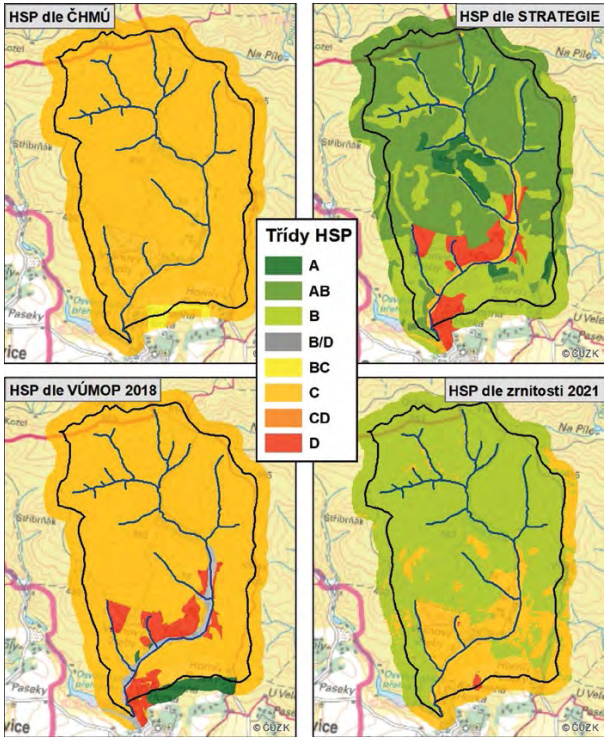
\includegraphics[height=12cm]{pictures/HSPmapa.png}
\caption{Plošné rozdělení jednotlivých HSP na povodí Hruškovice podle různých podkladů [16]}
\label{fig:hsp}
\end{figure}

\newpage
\newpage

\chapter{Použité technologie} \label{tehcnologie}

\section{Web Feature Service (WFS)} \label{wfs}
Web Feature Service je internetová služba pro šíření geografických informací, která nahradila šíření celých datových souborů například pomocí File Transporn Protocol (FTP). Služba je standardizována organizací Open Geospatial Consortium (OGC) v dokumentu  ISO 19119. [17] WFS je napsáno v jazyce XML a data jsou reprezentována primárně v jazyce GML. [18]

Na rozdíl od Web Map Service (WMS), která připojuje vrstvy jako needitovatelné rastrové podkladové vrstvy, WFS slouží ke sdílení vektorových dat s možností následné editace. Uživatel zašle požadavek ve formátu XML na WFS server, který vrátí odpověď opět V XML. [18]

\begin{figure}[ht] \label{obr5}
\centering
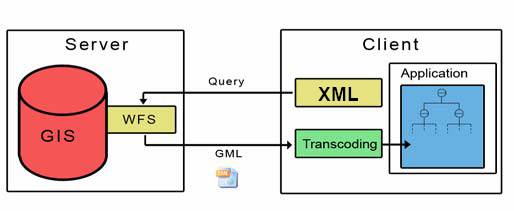
\includegraphics[height=6cm]{pictures/XML.png}
\caption{Schéma služby WFS [19]}
\label{fig:xml}
\end{figure}

Pro komunikaci se serverem poskytující WFS službu může uživatel využít následujících jedenáct operací:

\begin{table}[htbp]
  \centering
  \caption{Tabulka WFS operací} 
  \label{tab:WFS}
  \begin{tabular}{|c|c|p{7cm}|}
    \hline
    \textbf{Operace} & \textbf{Volitelný} & \textbf{Popis} \\
    \hhline{=|=|=}
    GetCapabilities & NE & Načte metadata o službě, včetně podporovaných operací a parametrů, a seznam dostupných typů prvků. \\
    \hline
    DescribeFeatureType & NE & Vrací popis struktury typů prvků a jejich vlastností, které WFS poskytuje nebo přijímá. \\
    \hline
    GetFeature & NE & Vrací výběr instancí prvků z datového úložiště publikovaného prostřednictvím WFS. \\
    \hline
    ListStoredQueries & NE & Vrací seznam dotazů, které byly uloženy v instanci WFS. \\
    \hline
    DescribeStoredQueries & NE & Vrací popis dotazů, které byly uloženy v instanci WFS. \\
    \hline
    GetPropertyValue & ANO & Načítá hodnotu vlastnosti prvku nebo část hodnoty složité vlastnosti pro sadu prvků. \\
    \hline
    GetFeatureWithLock & ANO & Podobné jako GetFeature, ale s možností uzamknout prvek pro následné úpravy. \\
    \hline
    LockFeature & ANO & Uzamkne sadu instancí prvků tak, aby je jiné operace nemohly měnit, dokud je zámek aktivní. \\
    \hline
    Transaction & ANO & Umožňuje modifikaci nebo odstranění instancí prvků a jejich vlastností. \\
    \hline
    CreateStoredQuery & ANO & Vytvoří a uloží dotaz, který může klient snadno vyvolat později. \\
    \hline
    DropStoredQuery & ANO & Odstraní dříve uložený dotaz ze serveru. \\
    \hline
  \end{tabular}
\end{table}

\section{YAML formát} \label{yaml}

\section{Python knihovna PyQt} \label{pyqt}
\section{Python knihovna pytest} \label{pytest}

\chapter{Postup implementace} \label{implementace}
\section{Tvorba grafického uživatelského rozhraní} \label{gui}
\section{Získávání vrstvy využití území (land use)} \label{landuse}
\section{analýza odtoků SCS-CN} \label{CN}
\clearpage  % SEM NESAHEJTE!
\addcontentsline{toc}{chapter}{Seznam použité literatury}  \label{zdroje}

\begin{thebibliography}{1}
\bibitem{MNYDGwleJOjKLRUp}
PONCE, V. M. and HAWKINS R. H. 1996. Runoff curve number: Has it reached maturity?
\textit{ Journal of Hydrologic Engineering 1(1):11-19. Dostupné z: \href{https://ponce.sdsu.edu/runoff11view.html}
{https://ponce.sdsu.edu/runoff11view.html}}

\bibitem{Holman2003}
HOLMAN, I.P.; HOLLIS, J.M.; BAMLEY, M.E. a THOMPSON, T.R.E. The contribution of soil structural degradation to catchment flooding: a preliminary investigation of the 2000 floods in England and Wales. \textit{Hydrology and earth system sciences}. 2003, roč. 7, č. 5, s.~754-765.

\bibitem{Lian2020}
LIAN, Huishu; YEN, Haw; HUANG, Jr-Chuan; FENG, Qingyu; QIN, Lihuan et al. CN-China: Revised runoff curve number by using rainfall-runoff events data in China. \textit{Water Research}. 2020, roč. 2020, č. 177, s.~115767. ISSN 0043-1354. Dostupné také z: \url{https://www.sciencedirect.com/science/article/pii/S0043135420303043}.

\bibitem{MNYDGwleJOjKdRUp}
JANEČEK, Miloslav. Ochrana zemědělské půdy před erozí: metodika.
\textit{ Praha: Powerprint, 2012. ISBN 978-80-87415-42-9. }

\bibitem{MNYDGwleJOjKLRU2}
KAVKA, Petr a KAŠPAR, Marek. Krátkodobé srážky pro hydrologické modelování a navrhování drobných vodohospodářských staveb v krajině: Certifikovaná metodika.
\textit{ Fakulta stavební ČVUT v Praze, 2023. ISBN 978-80-01-07115-1}

\bibitem{MNYDGwleJOjKLRU3}
JANEČEK, M. a P. KOVÁŘ. Aktuálnost „Metody čísel odtokových křivek –
CN“ k určování přímého odtoku z malého povodí.
\textit{ Vodní hospodářství. 2010,
č. 7, s. 187-189.} 

\bibitem{MNYDGwleJOjKLRU5}
Urban hydrology for small watersheds: Technical Release 55 (TR-55) (Second ed.).
\textit{ Natural Resources Conservation Service. Conservation Engineering Division, 1986.}


\bibitem{dONaeOjXanl1W2md}
ČSN P ISO/TS 19104, \textit{Geografická informace - Terminologie}. 2010.

\bibitem{Matejova2019}
MATEJOVÁ, Vlasta. \textit{Quantum GIS}. Diplomová práce. České Budějovice: Jihočeská univerzita v Českých Budějovicích, Ekonomická fakulta, 2019.

\bibitem{Baghdadi2018}
BAGHDADI, Nicolas; MALLET, Clément a ZRIBI, Mehrez. \textit{QGIS and Generic Tools}. Volume 1. John Wiley \& Sons, 2018. ISBN 9781119457091.

\bibitem{QPwvEntkWdxPk0Lz}
QGIS DEVELOPMENT TEAM. \textit{QGIS geographic information system}. Online. 2025. Dostupné z: \url{https://www.qgis.org}. [cit. 2025-01-26].

\bibitem{nEFEg7XpI9hVQCiO}
\textit{Katalog objektů ZABAGED®}. Verze 4.4. Zeměměřický úřad, 2024.


\bibitem{Devaty2018}
DEVÁTÝ, Jan. \textit{Klasifikace území pro erozní modely pomocí GIS a veřejně dostupných datových zdrojů}. Disertační práce. Praha: České vysoké učení technické v Praze, Fakulta stavební, Katedra hydromeliorací a krajinného inženýrství, 2018.

\bibitem{KocurBera2019}
KOCUR-BERA, Katarzyna. Data compatibility between the Land and Building Cadaster (LBC) and the Land Parcel Identification System (LPIS) in the context of area-based payments: A case study in the Polish Region of Warmia and Mazury. \textit{Land Use Policy}. 2019, roč. 2019, č. 80, s.~370-379. ISSN 0264-8377.

\bibitem{sSYEwLE0rNKoWGYk}
\textit{Nařízení vlády č. 307/2014 Sb. o stanovení podrobností evidence využití půdy podle uživatelských vztahů}. 2014. Dostupné také z: \url{http://www.zakonyprolidi.cz/cs/2014-307}.

\bibitem{Strouhal2022}
STROUHAL, Luděk a KAVKA, Petr. Hydrologické skupiny půd --- rozevřené nůžky hydrologických výpočtů (2. část). \textit{Vodní hospodářství}. 2022, roč. 72, č. 9, s.~7-12.

\bibitem{Vretanos2014}
VRETANOS, Panagiotis (Peter) A. \textit{OpenGIS Web Feature Service 2.0 Interface Standard --- With Corrigendum}. 2.0.2. Open Geospatial Consortium, 2014.

\bibitem{Zhang2005}
ZHANG, Chuanrong a LI, Weidong. The Roles of Web Feature and Web Map Services in Real-time Geospatial Data Sharing for Time-critical Applications. Online. \textit{Cartography and Geographic Information Science}. 2005, roč. 32, č. 4, s.~269-283. ISSN 1523-0406. Dostupné z: \url{https://doi.org/10.1559/152304005775194728}. [cit. 2025-02-25].

\bibitem{Schall2009}  
SCHALL, Gerhard, MENDEZ, Erick, KRUIJFF, Ernst, VEAS, Eduardo, JUNGHANNS, Sebastian, REITINGER, Bernhard a SCHMALSTIEG, Dieter.  
Handheld Augmented Reality for underground infrastructure visualization.  
\textit{Personal and Ubiquitous Computing}, 2009, roč. 13, s. 281-291.  
DOI: 10.1007/s00779-008-0204-5.  

\end{thebibliography}
\end{document}

